\begin{figure}[htbp]
  \centering
  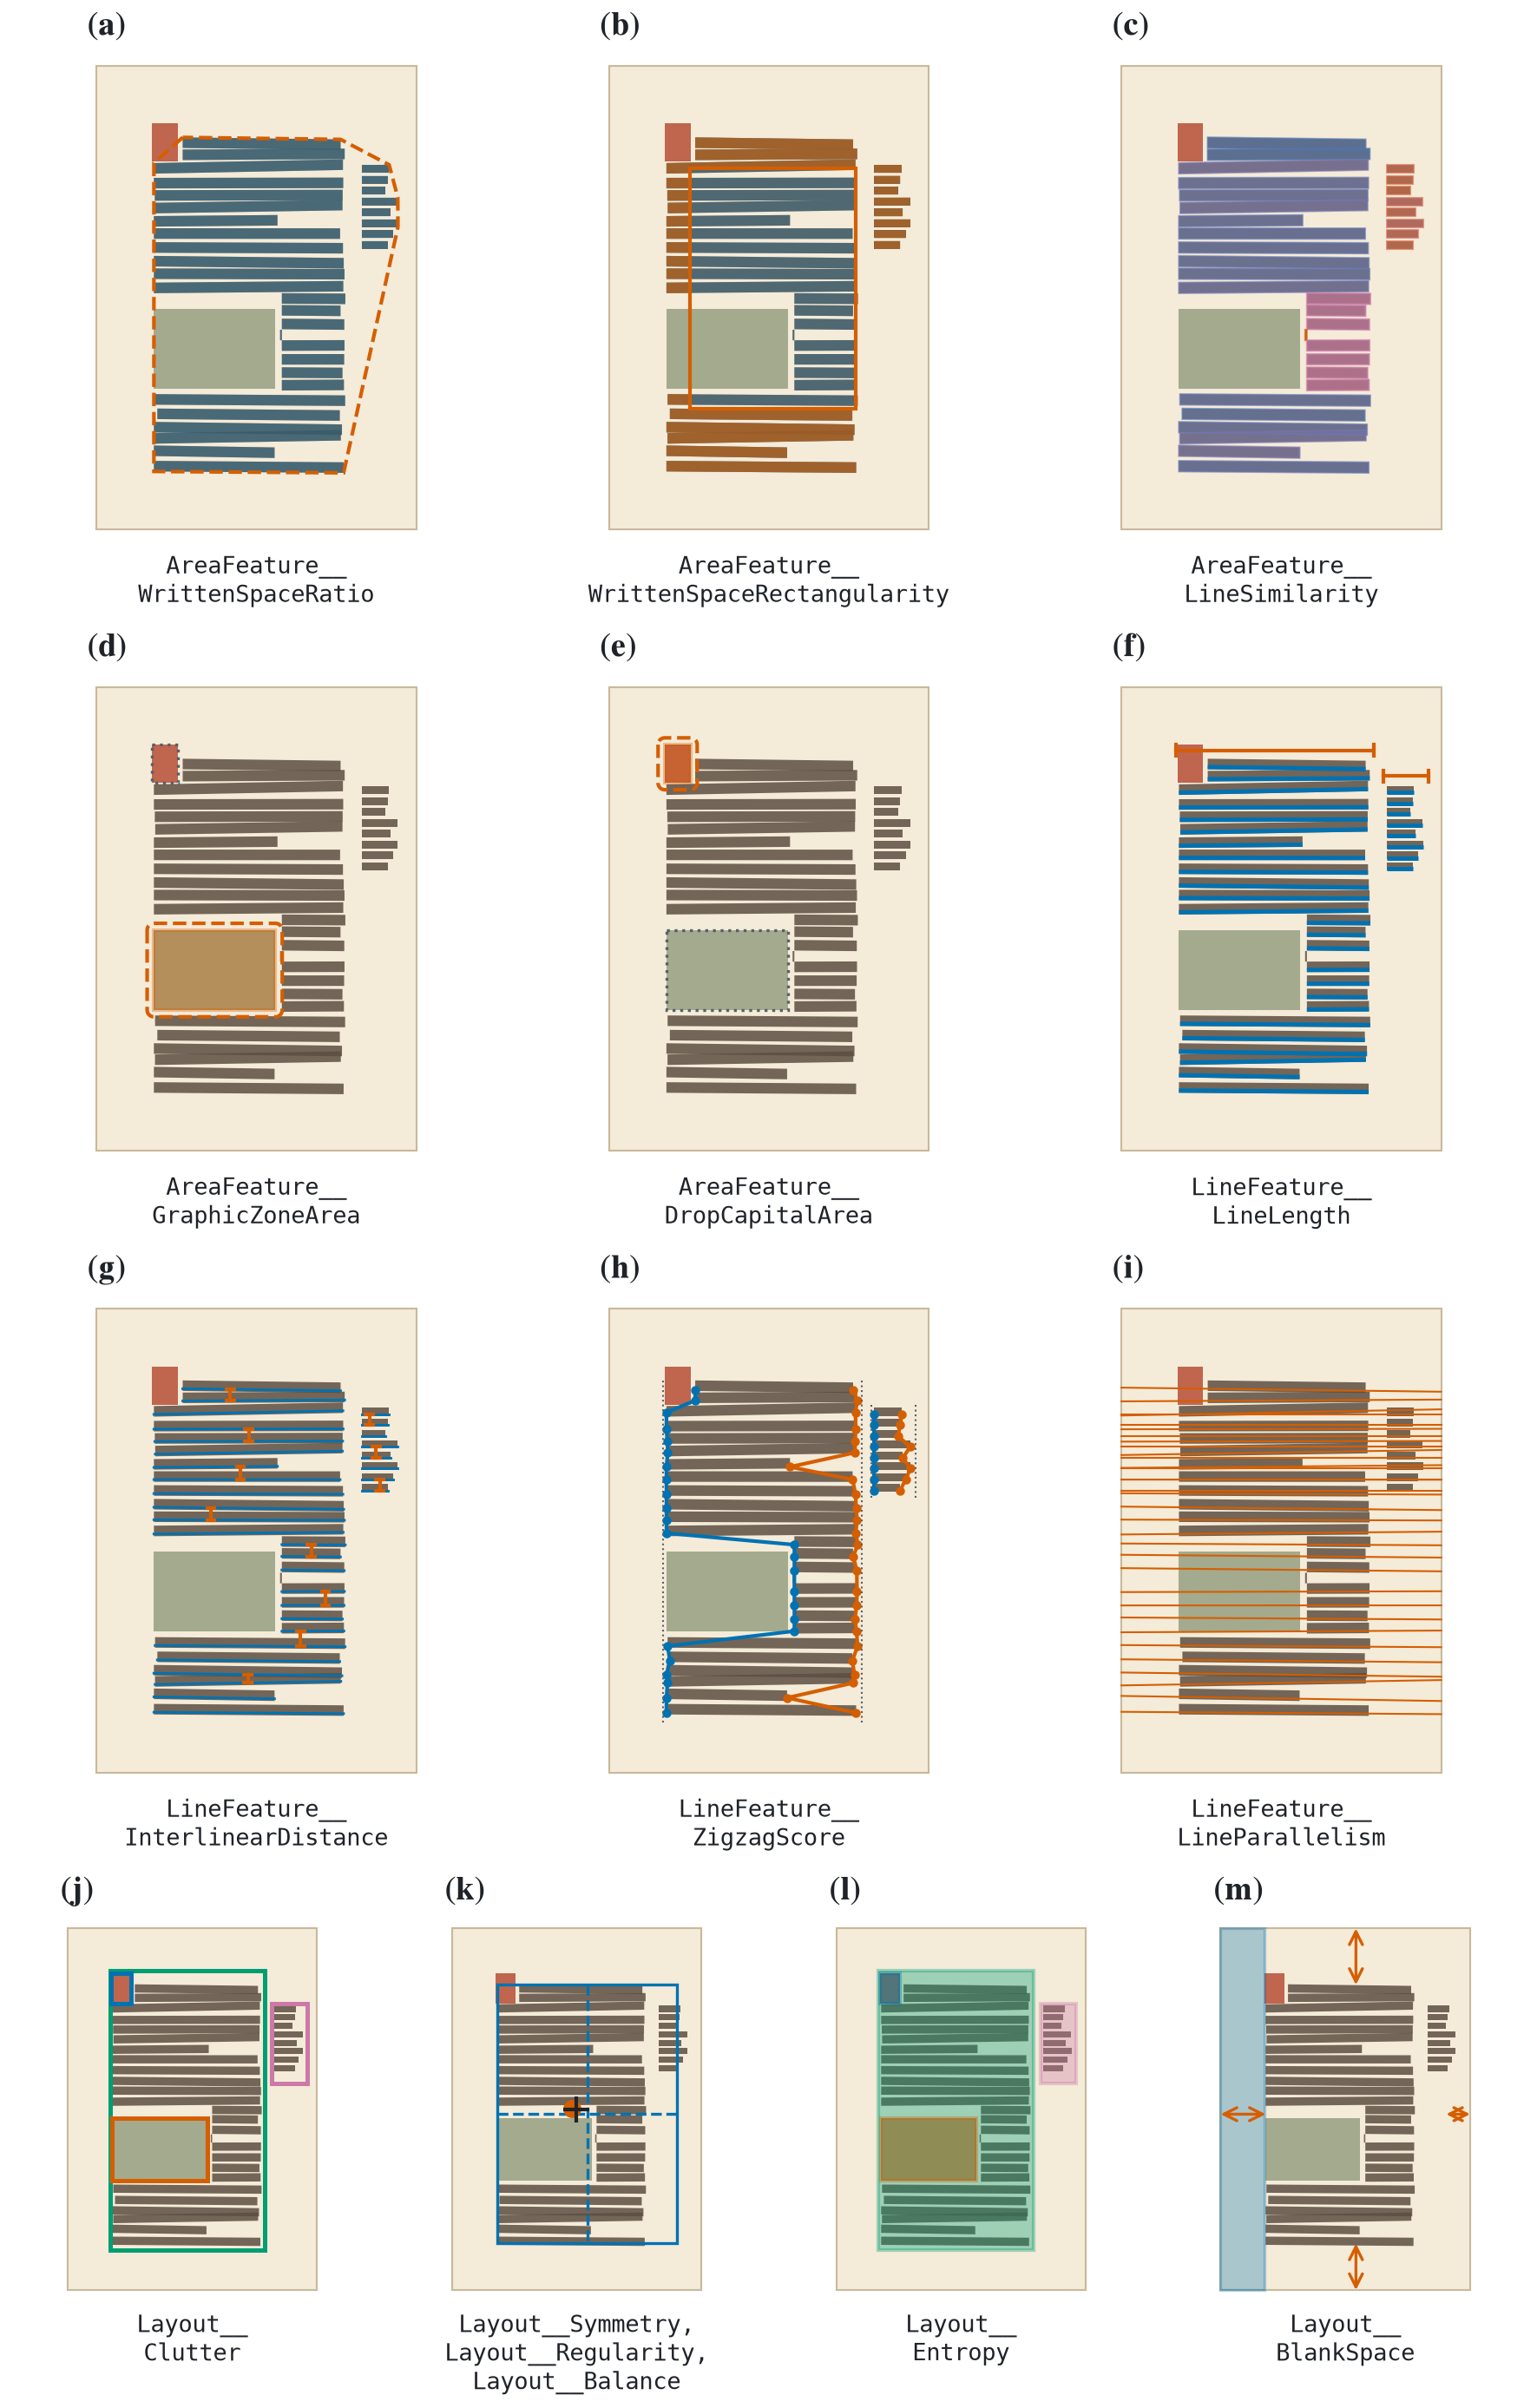
\includegraphics[width=15.00cm]{figures/geometry_feature_families.png}
  \caption{The features, each drawn on the same made-up page, with its code name below: the nine groups of geometric features, then the four measures of the Layout family. (a) WrittenSpaceRatio: the union of the line polygons (blue) and its convex hull (dashed); (b) WrittenSpaceRectangularity: the written space (blue), the rectangle of its area and the folio's proportions centred on it, and the written space outside it (vermillion); (c) LineSimilarity: each line coloured by its median Dice similarity with the other lines, their polygons centred on each other: blue where it is like most others, vermillion where it is unlike them; (d) GraphicZoneArea: the graphic zones (vermillion; drop capitals dotted grey); (e) DropCapitalArea: the drop capitals (vermillion; graphic zones dotted grey); (f) LineLength: the baselines measured (blue) and their zones' widths; (g) InterlinearDistance: the baselines and, for every third pair, the distance between them; (h) ZigzagScore: the lines' left (blue) and right (vermillion) ends, from line to line; (i) LineParallelism: each baseline's direction, drawn across the folio; (j) Clutter: the zones, outlined by type; (k) Order: the written mass's text block with its axes of symmetry, the mass's centre (dot) and the folio's (cross); (l) Entropy: the zones, filled by type; (m) Blank space: the largest empty rectangle and the margins around the text block.}
  \label{fig:geometry_feature_families}
\end{figure}
